\subsubsection{Compara\c c\~ao dos modelos}

A fim de ver melhor como cada modelo se comporta, os modelos foram comparados com base em um gráfico de violino, e assim observar qual dos modelos era o melhor.


\begin{figure}[H]
	\centering
	\caption{Comparação dos modelos ARIMAS}
	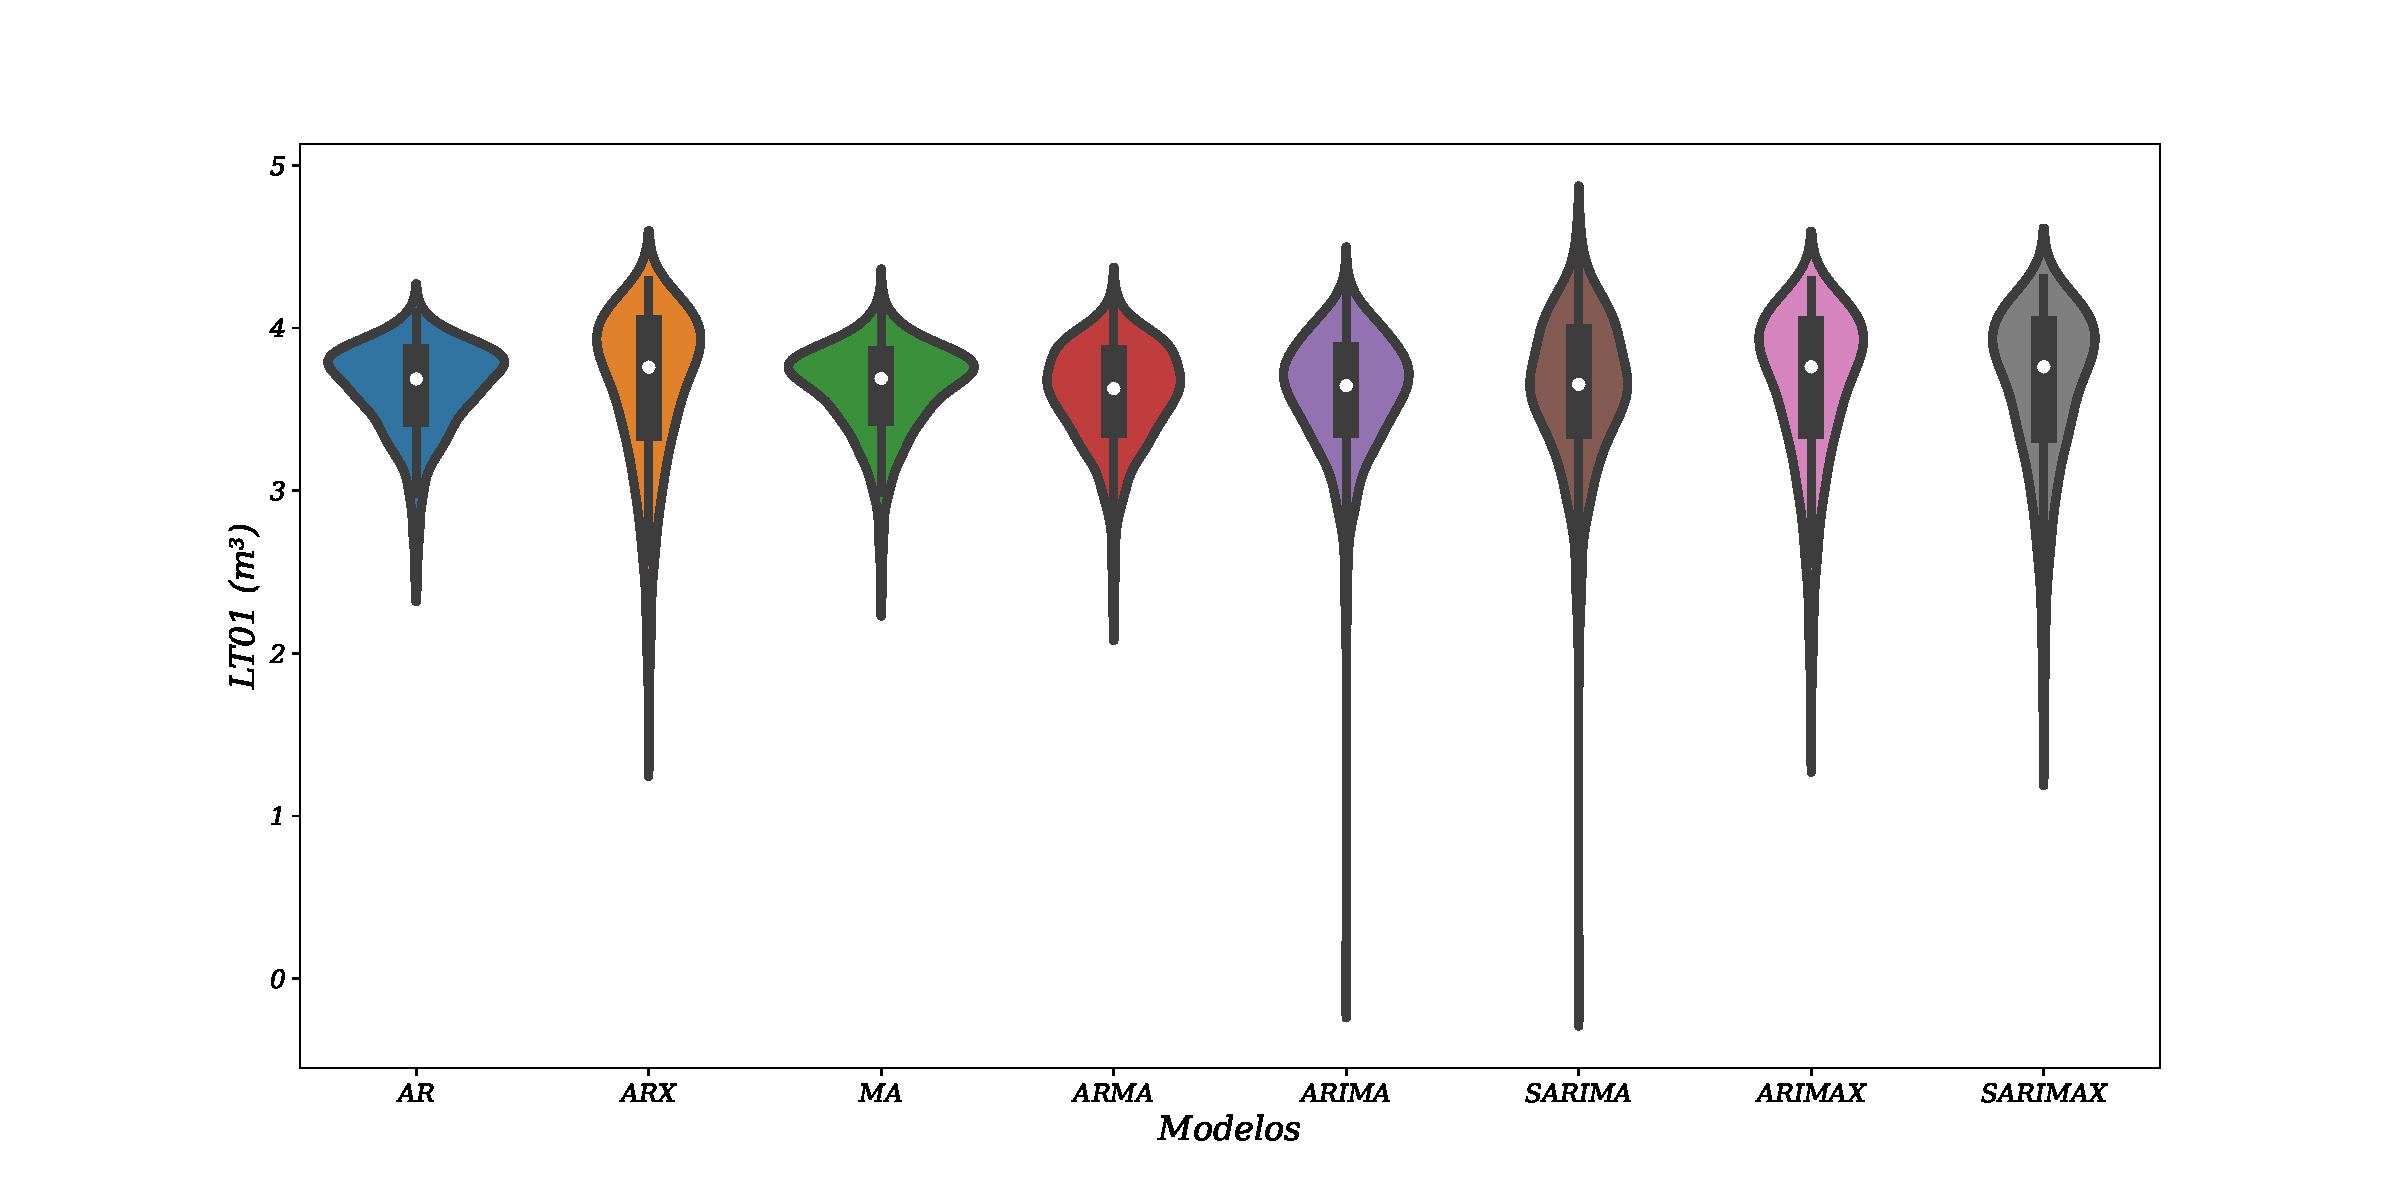
\includegraphics[width=0.9\linewidth]{Resultados/Figuras/modelos-arima}
	
	\label{fig:modelos-arima}
	
	Fonte: Elaboração própria a partir de dados da SANEPAR (2018 a 2020)
\end{figure}


\begin{figure}[H]
	\centering
	\caption{Comparação de modelos de regressão }
	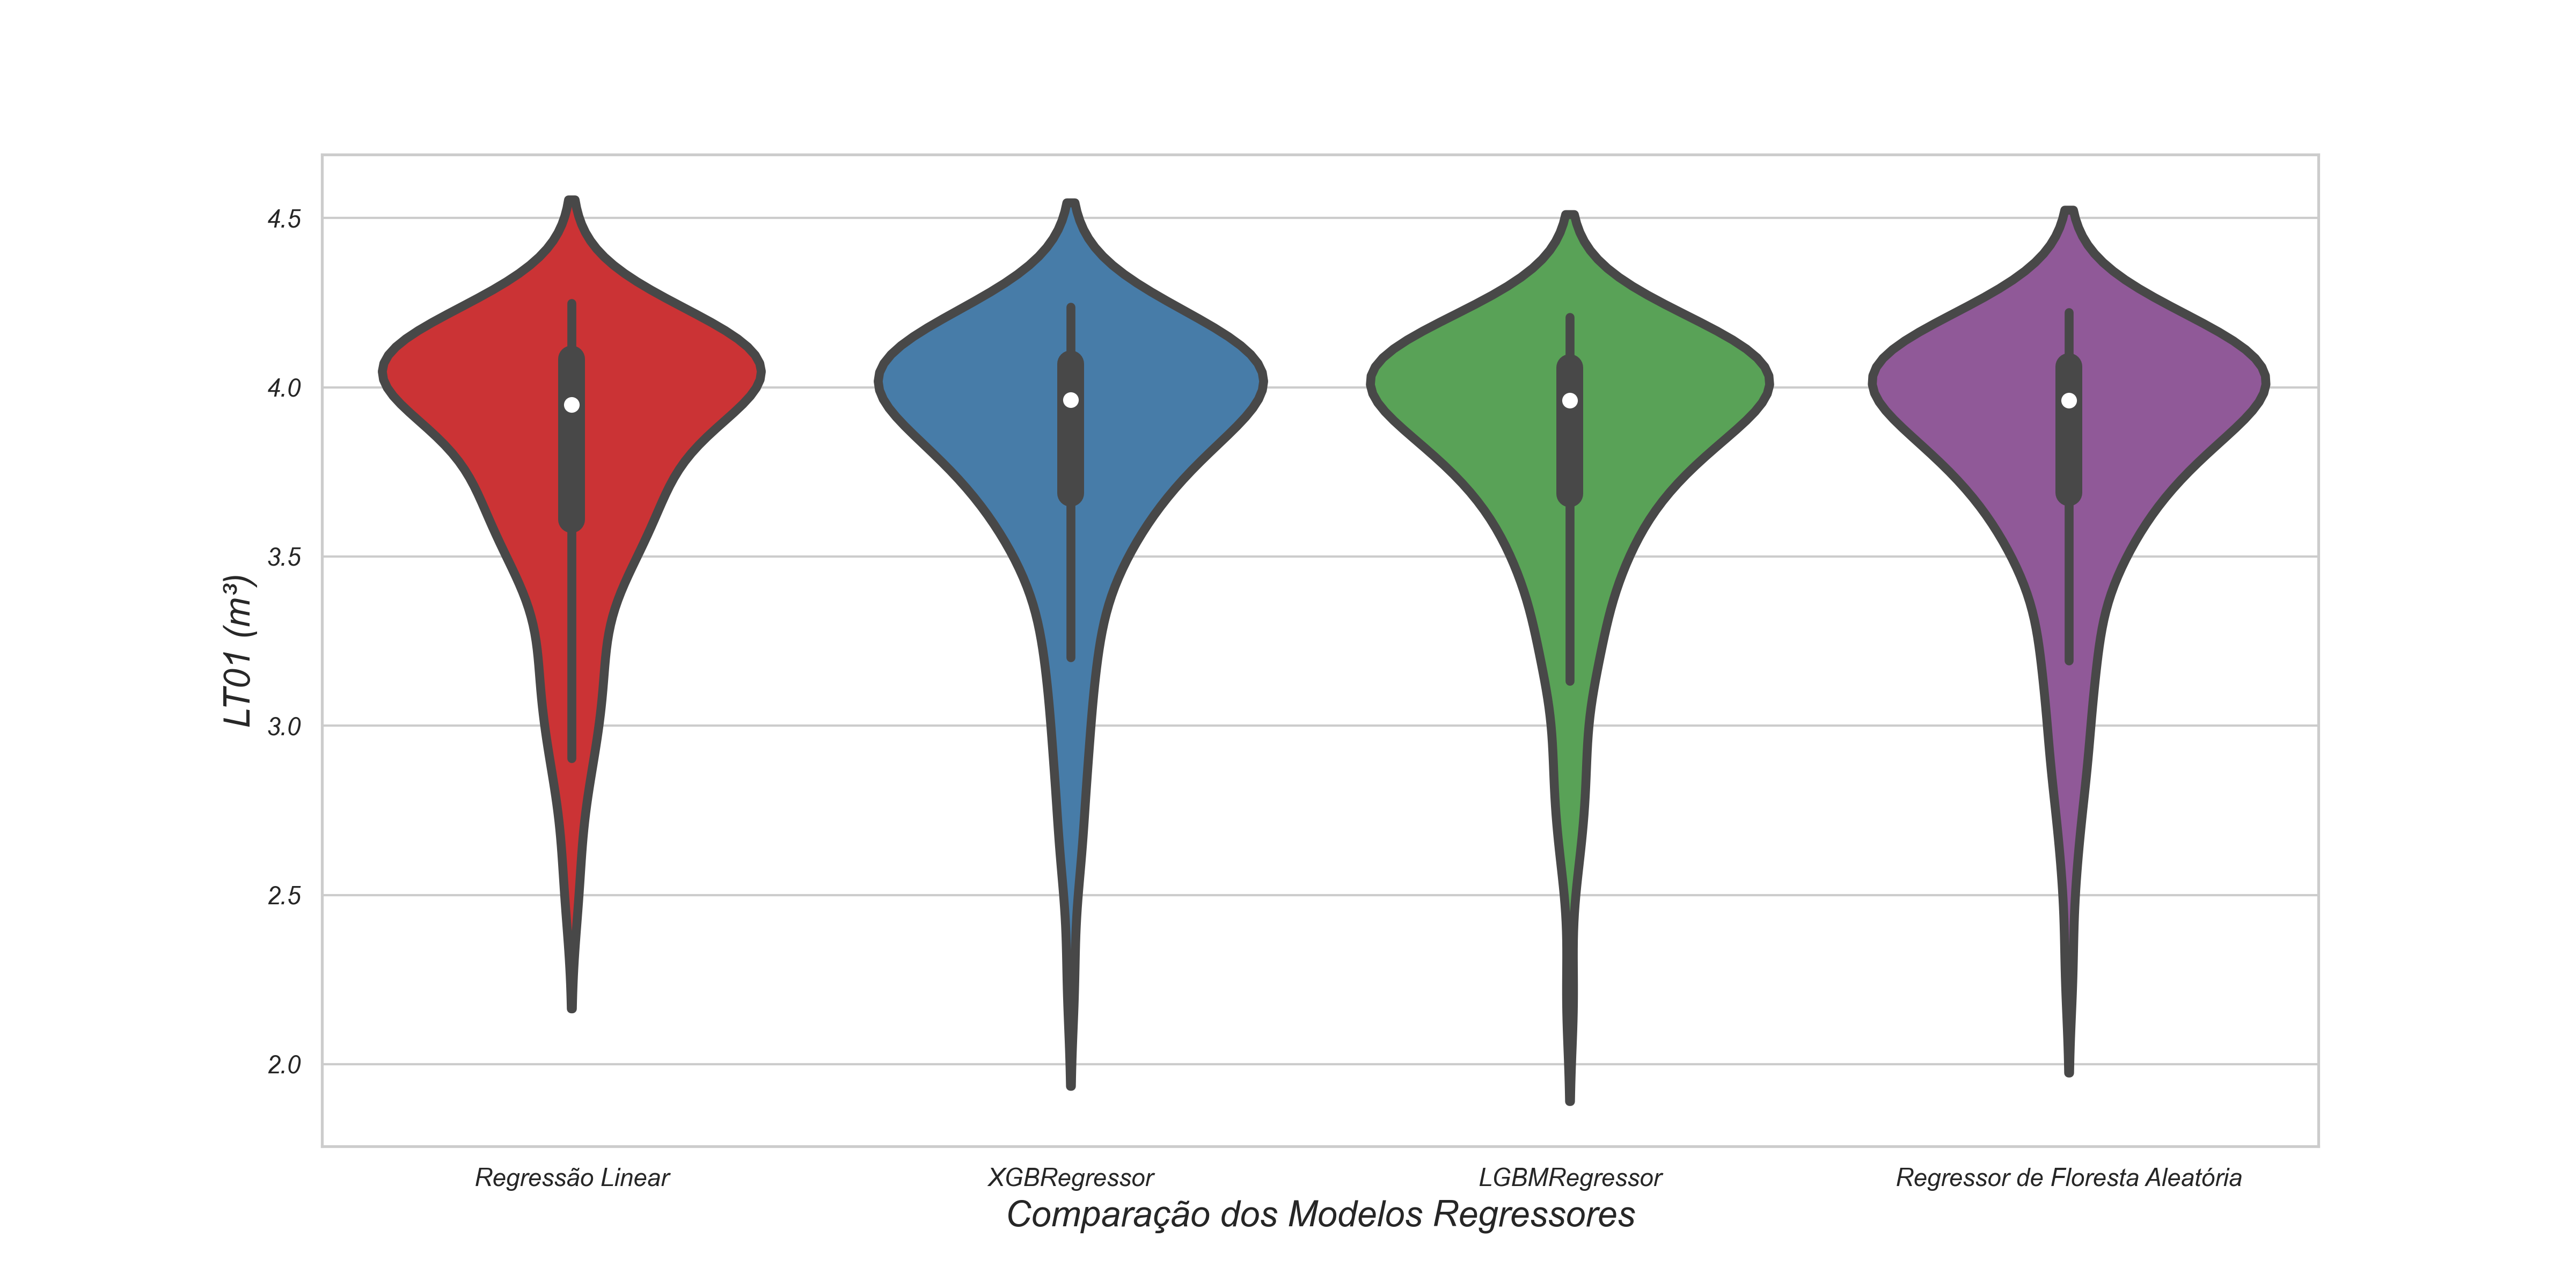
\includegraphics[width=0.9\linewidth]{Resultados/Figuras/violin-LR-XGB-LGBM-RF}
	
	\label{fig:violin-lr-xgb-lgbm-rf}
	
	Fonte: Elaboração própria a partir de dados da SANEPAR (2018 a 2020)
\end{figure}

Em comparação com os modelos apresentadosnas Figuras \ref{fig:modelos-arima} e \ref{fig:violin-lr-xgb-lgbm-rf} os modelos que podem ser observados que são os melhores levando em conta a modelagem dos dados nos modelos ARIMA os melhores são AR, ARX, MA, ARMA, ARIMAX e SARIMAX devido aos \textit{outliers} e ao limite inferior de alguns modelos que olham para os modelos de gradiente e regressão pode-se notar que eles eram semelhantes devido às técnicas de otimização matemática Grid Search (do inglês pesquisa grande) e Randomized Search (do inglês pesquisa aleatória) que permitiram o aperfeiçoamento do método utilizado. Em um horizonte de previsão pequeno, LR prevê melhor que os outros modelos, mas em um horizonte de previsão maior, XGBoost e Light GBM estão prevendo com melhor precisão. A floresta aleatória também está prevendo com precisão apenas atrás do XGBoost em previsões de longo prazo.

O método Ljung box é um método que pode ser estimado nos modelos ARIMAS de longo prazo se, a longo prazo, eles ainda irão prever eficientemente nos dados de longo prazo os modelos que melhor prevêem são os modelos ARX, ARIMAX e SARIMAX com as variáveis exógenas para modelos não lineares que podem aguentar mais tempo de previsão do que os outros modelos ARIMA.  
